\documentclass[12pt]{article}
\usepackage[utf8]{inputenc}
\usepackage{amsmath, amssymb}
\usepackage{hyperref}
\usepackage{tikz}
\usepackage[left=2.5cm,right=2.5cm,bottom=2.5cm]{geometry}
\usetikzlibrary{arrows, arrows.meta, positioning, bending, quotes}
\hypersetup{
    colorlinks=true}

\title{MATH 5707 (Spring 2026): Homework 6}
\date{}

\begin{document}
\vspace{-0.7in}

\maketitle
\vspace{-0.6in}


\section*{Directions and Introduction}
Submit a pdf of your solutions to the HW 6 assignment on Gradescope by 11:59 pm on March 27.

Problem 1 is marked as a peer review problem. \href{https://docs.google.com/document/d/1jSw9pmMJJFUx_6dTkcUi4k4HJNIrrIIgs9zdWhAycx0/edit?usp=sharing}{This document gives directions and deadlines for the peer review process.}



\section*{Problems}

\begin{enumerate}
\item[0.] If you would like any of these problems to be graded for proficiency with the key skills, list the skill and the corresponding problem.  If you want to label the sill by number, use the numbering that is in the syllabus.
  \item (Peer review problem; Bondy-Murty 5.1.5 (a); Each part will be worth 4 points and
graded as a separate problem.) A \emph{$k$-factor} of a graph $G$ is a $k$-regular spanning subgraph of $G$, and $G$ is \emph{$k$-factorable} if there are edge-disjoint $k$-factors $H_1$, $H_2,\ldots, H_n$ such that $G=H_1\cup H_2\cup\ldots \cup H_n$.  (In other words: $E(G)=E(H_1)\cup E(H_2)\cup\ldots \cup E(H_n)$ and $V(G)=V(H_1)=V(H_2)=\ldots =V(H_n)$.)
  \begin{enumerate}
  \item Show that $k_{n,n}$ and $k_{2n}$ are 1-factorable;
  \item Show that the Petersen graph is not $1$-factorable. 
 
  \end{enumerate}
    \item (Bondy-Murty 5.2.5)   A \emph{line} of a matrix is a row or a column of  the matrix. Show that the minimum number of  lines containing all the 1's of a (0, 1)-matrix is equal to the maximum number of 1's no two of which are in the same line. (Hint: Translate this problem into the language of vertex or edge covers on a graph.)
    \item Consider the bipartite graph $G$ shown below
    \begin{center}
    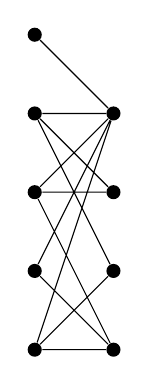
\begin{tikzpicture}
    \draw[every node/.style={inner sep=1.8pt,fill,circle}]
    (0,0) 
    \foreach \x in {0,1,2,3,4}{
    node(x\x) at (0,\x) {} }
    \foreach \y in {0,1,2,3}{ node (y\y) at (1,\y){}};
    \draw
    (x0)--(y1)--(x3)--(y3)--(x1)--(y0)--(x2)
    (x1)--(y3)--(x2)--(y3)--(x0)
    (x2)--(y2)--(x3)--(y3)--(x4)
    (x0)--(y0);
    \end{tikzpicture}
    \end{center}
    \begin{enumerate}
    \item Start with a matching $M$ such that $|M|=1$. Then, use the Hungarian algorithm to find a maximum matching on $G$. 
    \item Find the values of $\nu(G)$, $\tau(G)$, $\alpha(G)$, and $\rho(G)$.  
    \item Give an example of a minimum vertex cover and a maximum independent set in $G$. 
    \end{enumerate}

    \item Prove or disprove: A graph $G$ has a perfect matching if and only if $|N(S)|\ge |S|$ for all $S\subset V$. 

\end{enumerate}

\end{document}